\documentclass[12pt,letterpaper]{article}
\usepackage{fullpage}
\usepackage[top=2cm, bottom=4.5cm, left=2.5cm, right=2.5cm]{geometry}
\usepackage{amsmath,amsthm,amsfonts,amssymb,amscd}
\usepackage{lastpage}
\usepackage{enumerate}
\usepackage{fancyhdr}
\usepackage{mathrsfs}
\usepackage{xcolor}
\usepackage{graphicx}
\usepackage{listings}
\usepackage{hyperref}
\usepackage{tikz}
\usepackage{xfrac}
\usepackage{nicefrac}
\usepackage{xcolor}

\usetikzlibrary{shapes.geometric,fit}

\hypersetup{
    colorlinks=true,
    linkcolor=blue,
    linkbordercolor={0 0 1}
}

\setlength{\parindent}{0.0in}
\setlength{\parskip}{0.05in}

\newcommand\course{ECON 3211}
\newcommand\hwnumber{4}
\newcommand\NetIDa{dc3451}
\newcommand\NetIDb{David Chen}          

\theoremstyle{definition}
\newtheorem*{statement}{Statement}
\newtheorem*{claim}{Claim}
\newtheorem*{theorem}{Theorem}

\newcommand{\contra}{\Rightarrow\!\Leftarrow}
\newcommand{\Lag}{\mathcal{L}}

\pagestyle{fancyplain}
\headheight 35pt
\lhead{\NetIDa}
\lhead{\NetIDa\\\NetIDb}
\chead{\textbf{\Large Problem Set \hwnumber}}
\rhead{\course \\ \today}
\lfoot{}
\cfoot{}
\rfoot{\small\thepage}
\headsep 1.5em

\begin{document}

\section*{Problem 1}

\subsection*{a)}

The consumer would never consume at a corner of their budget constraint. This is
true in general of Cobb-Douglass utility functions, as taking either quantity as
0 would vanish utility. Thus, in any case, they consume at least some of either
good, as we take the goods to be perfectly divisible.

\subsection*{b)}

We simply can note that the problem is symmetric across $q_x, q_y$ and conclude
that equal quantities must be bought, and thus $q_x^* = q_y^* = 4$.

However, I suspect that this may not be satisfactory for the TA's. The problem
then is $\max[q_x^{0.5}q_y^{0.5}]$ over $q_x,q_y$, such that $2q_x + 2q_y = 16$.

\begin{alignat*}{2}
  && \Lag(q_x,q_y,\lambda) &= q_x^{\frac{1}{2}}q_y^{\frac{1}{2}} - \lambda(p_xq_x + p_yq_y - M) \\
  && \frac{\delta \Lag}{\delta q_x} &= \frac{1}{2}(\frac{q_y}{q_x})^{\frac{1}{2}} -
  p_x\lambda = 0 \\
  && \frac{\delta \Lag}{\delta q_y} &= \frac{1}{2}(\frac{q_x}{q_y})^{\frac{1}{2}} -
  p_y\lambda = 0\\
  && \frac{\delta \Lag}{\delta \lambda} &= -p_xq_x - p_yq_y + M = 0 \\
  &\implies& \frac{q_y^*}{q_x^*} &= \frac{p_x}{p_y} \\
  &\implies& q_y^* &= \frac{p_xq_x^*}{p_y} \\
  &\implies& 2p_xq_x^* &= M \\
  &\implies& q_x^* &= \frac{M}{2p_x} = 4\\
  &\implies& q_y^* &= \frac{M}{2p_y} = 4
\end{alignat*}

The consumer has utility $\overline{U} = (4)^{0.5}(4)^{0.5} = 4$.

\subsection*{c)}
\subsubsection*{c.1}

The cost of the original bundle would be $8(4) + 2(4) = 40$.

\subsubsection*{c.2}

Her utility function remains the same, so she would purchase then $q_x =
\frac{40}{2(8)} = 2.5, q_y = \frac{40}{2(2)} = 10$.

\subsubsection*{c.3}

The difference in good $x$ is $2.5 - 4 = -1.5$, as the Slutsky bundle has
$1.5$ units of $x$ less (own substitution).

\subsubsection*{c.4}

The difference in good $y$ is $10 - 4 = 6$, as the Slutsky bundle has
$6$ units of $y$ more (cross substitution).

\subsubsection*{d.1}

The new optimal bundle is at $q_x = \frac{16}{2(8)} = 1, q_y = \frac{16}{2(2)} =
  4$.

\subsubsection*{d.2}

The difference in good $x$ is $1 - 2.5 = -1.5$, such that the new optimal bundle
has $1.5$ units of $x$ less (own income).

\subsubsection*{d.3}

The difference in good $y$ is $4 - 10 = -6$, such that the new optimal bundle
has $6$ units of $x$ less (cross income).

\subsection*{e)}

\begin{center}
  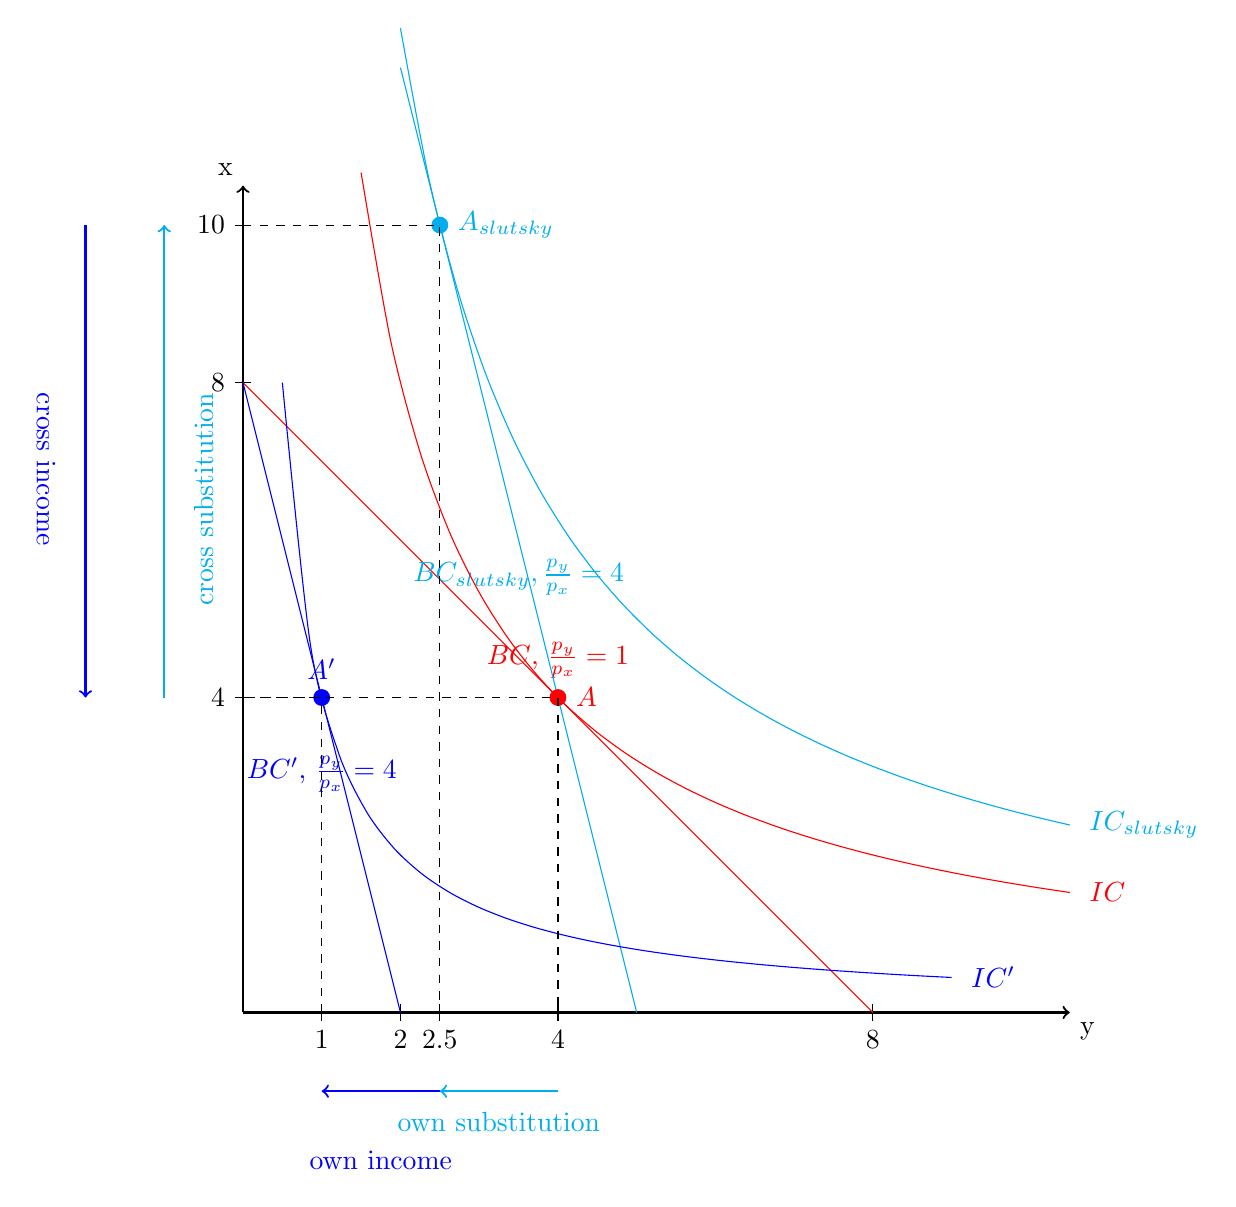
\begin{tikzpicture}[
    dot/.style={shape=circle, inner sep=2pt, draw, node contents=},
    circ/.style={shape=circle, inner sep=2pt, draw, fill}]
    \draw[thick,->] (0,0) -- (10.5,0) node[anchor=north west] {y};
    \draw[thick,->] (0,0) -- (0,10.5) node[anchor=south east] {x};
    
    \draw (4cm,3pt) -- (4cm,-3pt) node[anchor=north] {$4$}; 
    \draw (1cm,3pt) -- (1cm,-3pt) node[anchor=north] {$1$}; 
    \draw (2cm,3pt) -- (2cm,-3pt) node[anchor=north] {$2$}; 
    \draw (2.5cm,3pt) -- (2.5cm,-3pt) node[anchor=north] {$2.5$}; 
    \draw (8cm,3pt) -- (8cm,-3pt) node[anchor=north] {$8$}; 

    \draw (3pt,4cm) -- (-3pt,4cm) node[anchor=east] {$4$};
    \draw (3pt,8cm) -- (-3pt,8cm) node[anchor=east] {$8$};
    \draw (3pt,10cm) -- (-3pt,10cm) node[anchor=east] {$10$};

    \draw[color=red] (0,8) -- node[label=above:{$BC$, $\frac{p_y}{p_x} = 1$}]{} (8,0);
    \draw[color=blue] (0,8) -- node[label=below:{$BC'$, $\frac{p_y}{p_x} = 4$},yshift=-5mm]{} (2,0);
    \draw[color=cyan] (2, 12) -- node[label=below:{$BC_{slutsky}, \frac{p_y}{p_x}=4$}]{} (5,0);

    % \draw[color=red] plot[smooth] coordinates { (1.5,10.7) (2,8) (4,4) (8,2) (10.7, 1.5) } node[label=right:{$IC$}]{};

    \draw[color=red,domain=1.5:10.5,smooth,variable=\x] plot ({\x},{16/\x}) node[label=right:{$IC$}]{};
    \draw[color=blue,domain=0.5:9,smooth,variable=\x] plot ({\x},{4/\x})node[label=right:{$IC'$}]{};
    \draw[color=cyan,domain=2:10.5,smooth,variable=\x] plot ({\x},{25/\x})node[label=right:{$IC_{slutsky}$}]{};
    % \draw[color=blue] plot[smooth] coordinates {(0.5,8) (1,4) (1.5,2.7) (2,2) (2.7, 1.5) (4,1) (8, 0.5)}node[label=right:{$IC'$}]{};
    % \draw[color=cyan] plot[smooth] coordinates { (2,12.5) (2.25,11.2) (2.5,10) (3,8.4) (5,5) (8.3,3) (10, 2.5) }node[label=right:{$IC_{slutsky}$}]{};

    
    \draw[color=blue] (1,4) node[circ,label=above:{$A'$}]{};
    \draw[color=cyan] (2.5,10) node[circ,label=right:{$A_{slutsky}$}]{};
    \draw[color=red] (4,4) node[circ,label=right:{$A$}]{};

    \draw[dashed] (1,0) -- (1,4) -- (0,4);
    \draw[dashed] (0,4) -- (4,4) -- (4,0);
    \draw[dashed] (0,10) -- (2.5,10) -- (2.5,0);

    \draw[color=cyan,->,thick] (4, -1) -- node[label=below:{own substitution}]{} (2.5, -1);
    \draw[color=blue,->,thick] (2.5,-1) -- node[label=below:{own income},yshift=-5mm]{} (1, -1);

    \draw[color=cyan,->,thick] (-1, 4) -- node[midway,left,yshift=10mm,xshift=5mm,rotate=90]{cross substitution} (-1, 10);
    \draw[color=blue,->,thick] (-2,10) -- node[midway,right,yshift=10mm,xshift=-5mm,rotate=270]{cross income} (-2, 4);
  \end{tikzpicture}
\end{center}

\subsection*{f)}

\begin{center}
  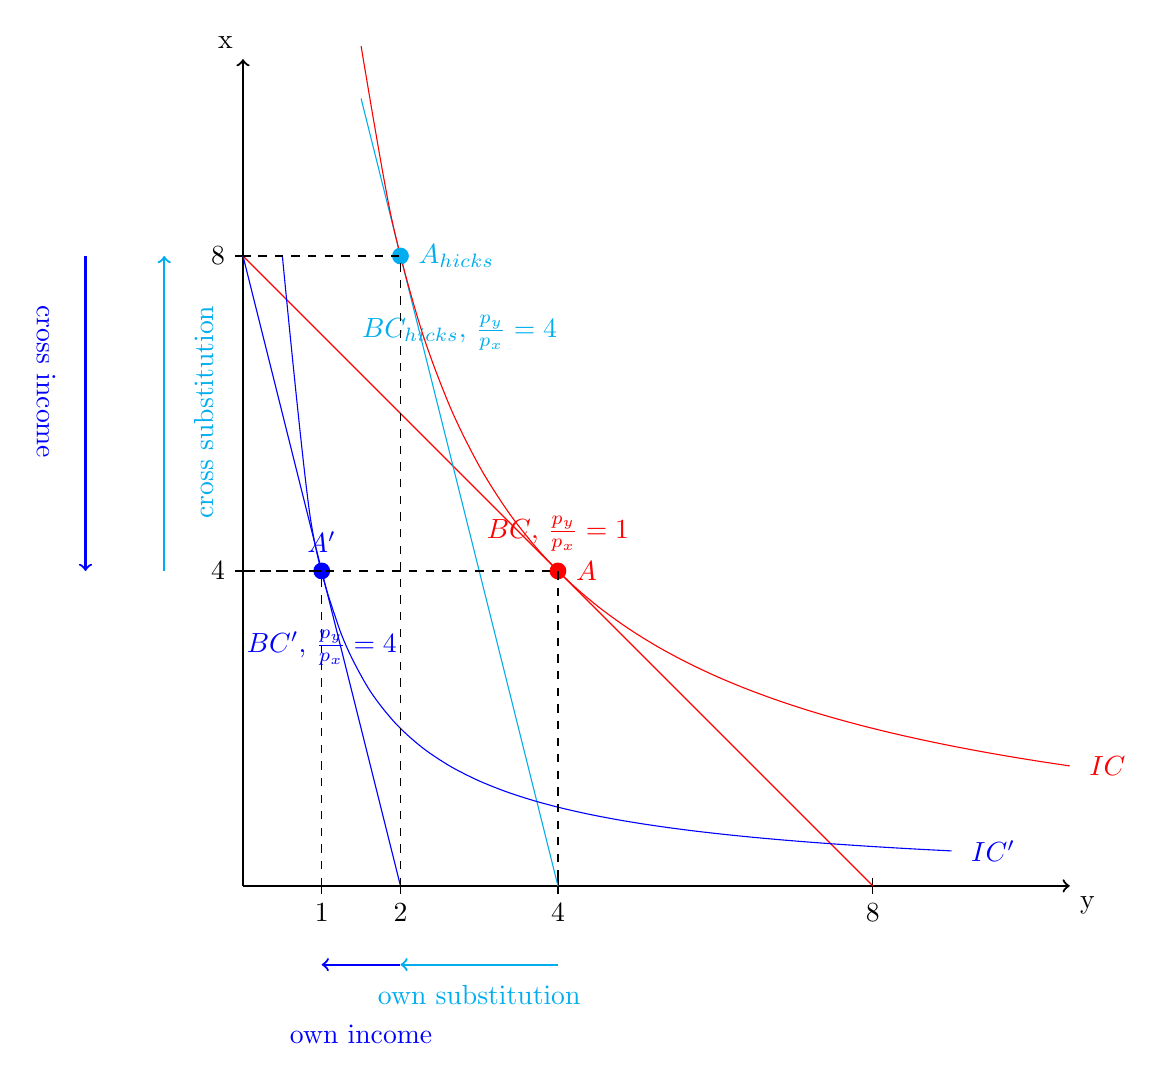
\begin{tikzpicture}[
    dot/.style={shape=circle, inner sep=2pt, draw, node contents=},
    circ/.style={shape=circle, inner sep=2pt, draw, fill}]
    \draw[thick,->] (0,0) -- (10.5,0) node[anchor=north west] {y};
    \draw[thick,->] (0,0) -- (0,10.5) node[anchor=south east] {x};
    
    \draw (4cm,3pt) -- (4cm,-3pt) node[anchor=north] {$4$}; 
    \draw (1cm,3pt) -- (1cm,-3pt) node[anchor=north] {$1$}; 
    \draw (2cm,3pt) -- (2cm,-3pt) node[anchor=north] {$2$}; 
    \draw (8cm,3pt) -- (8cm,-3pt) node[anchor=north] {$8$}; 

    \draw (3pt,4cm) -- (-3pt,4cm) node[anchor=east] {$4$};
    \draw (3pt,8cm) -- (-3pt,8cm) node[anchor=east] {$8$};

    \draw[color=red] (0,8) -- node[label=above:{$BC$, $\frac{p_y}{p_x} = 1$}]{} (8,0);
    \draw[color=blue] (0,8) -- node[label=below:{$BC'$, $\frac{p_y}{p_x} = 4$},yshift=-5mm]{} (2,0);
    \draw[color=cyan] (1.5,10) -- node[label=below:{$BC_{hicks}$, $\frac{p_y}{p_x} = 4$},yshift=25mm]{} (4,0);

    % \draw[color=red] plot[smooth] coordinates { (1.5,10.7) (2,8) (4,4) (8,2) (10.7, 1.5) } node[label=right:{$IC$}]{};
    % \draw[color=blue] plot[smooth] coordinates {(0.5,8) (1,4) (1.5,2.7) (2,2) (2.7, 1.5) (4,1) (8, 0.5)}node[label=right:{$IC'$}]{};

    \draw[color=red,domain=1.5:10.5,smooth,variable=\x] plot ({\x},{16/\x}) node[label=right:{$IC$}]{};
    \draw[color=blue,domain=0.5:9,smooth,variable=\x] plot ({\x},{4/\x}) node[label=right:{$IC'$}]{};

    
    \draw[color=blue] (1,4) node[circ,label=above:{$A'$}]{};
    \draw[color=red] (4,4) node[circ,label=right:{$A$}]{};
    \draw[color=cyan] (2,8) node[circ,label=right:{$A_{hicks}$}]{};

    \draw[dashed] (1,0) -- (1,4) -- (0,4);
    \draw[dashed] (2,0) -- (2,8) -- (0,8);
    \draw[dashed] (0,4) -- (4,4) -- (4,0);

    \draw[color=cyan,->,thick] (4, -1) -- node[label=below:{own substitution}]{} (2, -1);
    \draw[color=blue,->,thick] (2,-1) -- node[label=below:{own income},yshift=-5mm]{} (1, -1);

    \draw[color=cyan,->,thick] (-1, 4) -- node[midway,left,yshift=15mm,xshift=5mm,rotate=90]{cross substitution} (-1, 8);
    \draw[color=blue,->,thick] (-2,8) -- node[midway,right,yshift=15mm,xshift=-5mm,rotate=270]{cross income} (-2, 4);
  \end{tikzpicture}
\end{center}

\subsection*{g)}

\subsubsection*{g.1}

To find the Hicksian bundle, we have that $U(q_x,q_y) = 4$, and that the Hicks line
has slope $-\frac{p_q}{p_x} = -4$. Then $\frac{dq_x}{dq_y} =
-\frac{(\frac{q_y}{q_x})^{\frac{1}{2}}}{(\frac{q_x}{q_y})^{\frac{1}{2}}} = -\frac{q_y}{q_x}$
along $U(q_x,q_y) = 4$. Thus, we have that $\frac{q_y}{q_x} = 4 \implies q_y= 4q_x$. In
order to have $U(q_x,4q_x) = 2q_x = 4$, we must have $q_x^* = 2, q_y^* = 8$. 

\subsubsection*{g.2}

The own substitution effect is $2-4 = -2$, as there are $2$ less units of $x$ in
the Hicksian bundle. The cross substitution effect is $8-4=4$, as there are $4$
more units of good $y$ in the Hicksian bundle.

\subsubsection*{g.3}

The own income effect is $1-2=-1$, as there is $1$ less unit of $x$ in the new
optimal bundle from the Hicksian bundle. Similarly, since there are $4$ less
units of $y$, we have that the cross income effect is $4-8 = -4$.

\section*{Problem 2}

\subsection*{a)}

The optimization problem faced is to $\max[q_R^{\frac{1}{2}}q_B^{\frac{1}{2}}]$ over
$q_R,q_B$, such that $P_Rq_R + P_Bq_B = M$.

\subsection*{b)}

This is identical to the system in problem 1, given a few name changes.

\subsubsection*{b.1}
\begin{alignat*}{2}
  && \Lag(q_R,q_B,\lambda) &= q_R^{\frac{1}{2}}q_B^{\frac{1}{2}} - \lambda(P_Rq_R + P_Bq_B - M) \\
\end{alignat*}
\subsubsection*{b.2}
\begin{alignat*}{2}
  && \frac{\delta \Lag}{\delta q_R} &= \frac{1}{2}(\frac{q_B}{q_R})^{\frac{1}{2}} -
  P_R\lambda = 0 \\
  && \frac{\delta \Lag}{\delta q_B} &= \frac{1}{2}(\frac{q_R}{q_B})^{\frac{1}{2}} -
  P_B\lambda = 0\\
  && \frac{\delta \Lag}{\delta \lambda} &= -P_Rq_R - P_Bq_B + M = 0 \\
\end{alignat*}
\subsubsection*{b.3}
\begin{alignat*}{2}
  &\implies& \frac{q_B^*}{q_R^*} &= \frac{P_R}{P_B} \\
  &\implies& q_B^* &= \frac{P_Rq_R^*}{P_B} \\
  &\implies& 2P_Rq_R^* &= M \\
  &\implies& q_R^* &= \frac{M}{2P_R}\\
  &\implies& q_B^* &= \frac{M}{2P_B} \\
  &\implies& \lambda &= \frac{1}{2(P_RP_B)^{\frac{1}{2}}}
\end{alignat*}

\subsubsection*{b.4}

\begin{align*}
  V(P_B,P_R,M) &= (\frac{M}{2P_R})^{\frac{1}{2}}(\frac{M}{2P_B})^{\frac{1}{2}}
  \\
               &= \frac{M}{2(P_RP_B)^{\frac{1}{2}}}
\end{align*}

\subsection*{c)}

His optimal bundle is $q_R^* = \frac{M}{2P_R} = \frac{2400}{2(200)} = 6, q_B^* =
\frac{M}{2P_B} = \frac{2400}{2(50)} = 24$.

His indirect utility is $V_0 = \frac{2400}{2\sqrt{50(200)}} = 12$

\subsection*{d)}

The current cost of his optimal bundle is $6(120) + 24(80) = \$2640$, which is
not affordable.

This however is not the optimal bundle at the other town, which is $q_R^* =
\frac{2400}{2(120)} = 10, q_B^* = \frac{2400}{2(80)} = 15$ at a cost equal to $M
= 2400$.

\subsection*{e)}

$V(120,80,2400) = \frac{2400}{2(120(80))^{\frac{1}{2}}} =
\frac{1200}{40\sqrt{6}} =\frac{30}{\sqrt{6}} = 5\sqrt{6} \approx 12.25$.

\subsection*{f)}

Roger's utility is higher when shopping in the other town rather than the local town.

\subsection*{g)}

\subsubsection*{g.1}

$V(200,50,2400) = 12 = V(120,80,2400+CV)$.

\begin{alignat*}{2}
  && V(120,80,2400+CV) &= \frac{2400 + CV}{2(120(80))^{\frac{1}{2}}} \\
  &\implies& 12 &= \frac{2400 + CV}{2(40)\sqrt{6}} \\
  &\implies& 960\sqrt{6} &= 2400 + CV \\
  &\implies& CV &= 960\sqrt{6} - 2400 = -\$48.49
\end{alignat*}

It is negative to indicate willingness to pay to get access to the new bundle.

(Although this is taken to be positive in recitation for some reason?)

\subsubsection*{g.2i}

The problem is to $\min[120q_R + 80q_B]$ over $q_R,q_B$, such that
$q_R^{\frac{1}{2}}q_B^{\frac{1}{2}} = 12$.

\subsubsection*{g.2ii}

\begin{align*}
  \Lag(q_R,q_B,\lambda) &= 120q_R + 80q_B - \lambda(q_R^{\frac{1}{2}}q_B^{\frac{1}{2}} - 12) \\
\end{align*}

\subsubsection*{g.2iii}

\begin{align*}
  \frac{\delta \Lag}{\delta q_R} &= 120 - \frac{\lambda}{2}(\frac{q_B}{q_R})^{\frac{1}{2}} = 0 \\
  \frac{\delta \Lag}{\delta q_B} &= 80 - \frac{\lambda}{2}(\frac{q_R}{q_B})^{\frac{1}{2}} = 0 \\
  \frac{\delta \Lag}{\delta \lambda} &= q_R^{\frac{1}{2}}q_B^{\frac{1}{2}} - 12 = 0 \\
\end{align*}

\subsubsection*{g.2iv}

\begin{alignat*}{2}
  && \frac{q_B}{q_R} &= \frac{120}{80} \\
  &\implies& q_B &= \frac{3}{2}q_R \\
  &\implies& (\frac{3}{2})^{\frac{1}{2}}q_R &= 12 \\
  &\implies& q_R &= 12(\frac{2}{3})^{\frac{1}{2}} = 4\sqrt{6} \\
  &\implies& q_B &= 12(\frac{3}{2})^{\frac{1}{2}} = 6\sqrt{6} \\
  &\implies& \lambda &= 80(2(\frac{3}{2})^{\frac{1}{2}}) = 80\sqrt{6} 
\end{alignat*}

\subsubsection*{g.2v}

The cheapest bundle costs $120(4\sqrt{6}) + 80(6\sqrt{6}) = 960\sqrt{6}$.
Roger's compensating variation is then $960\sqrt{6} - 2400 = -\$48.49$.

\section*{Problem 3}

\subsection*{\textcolor{red}{a),} \textcolor{blue}{b), c),} d), \textcolor{cyan}{e)}}

\begin{center}
  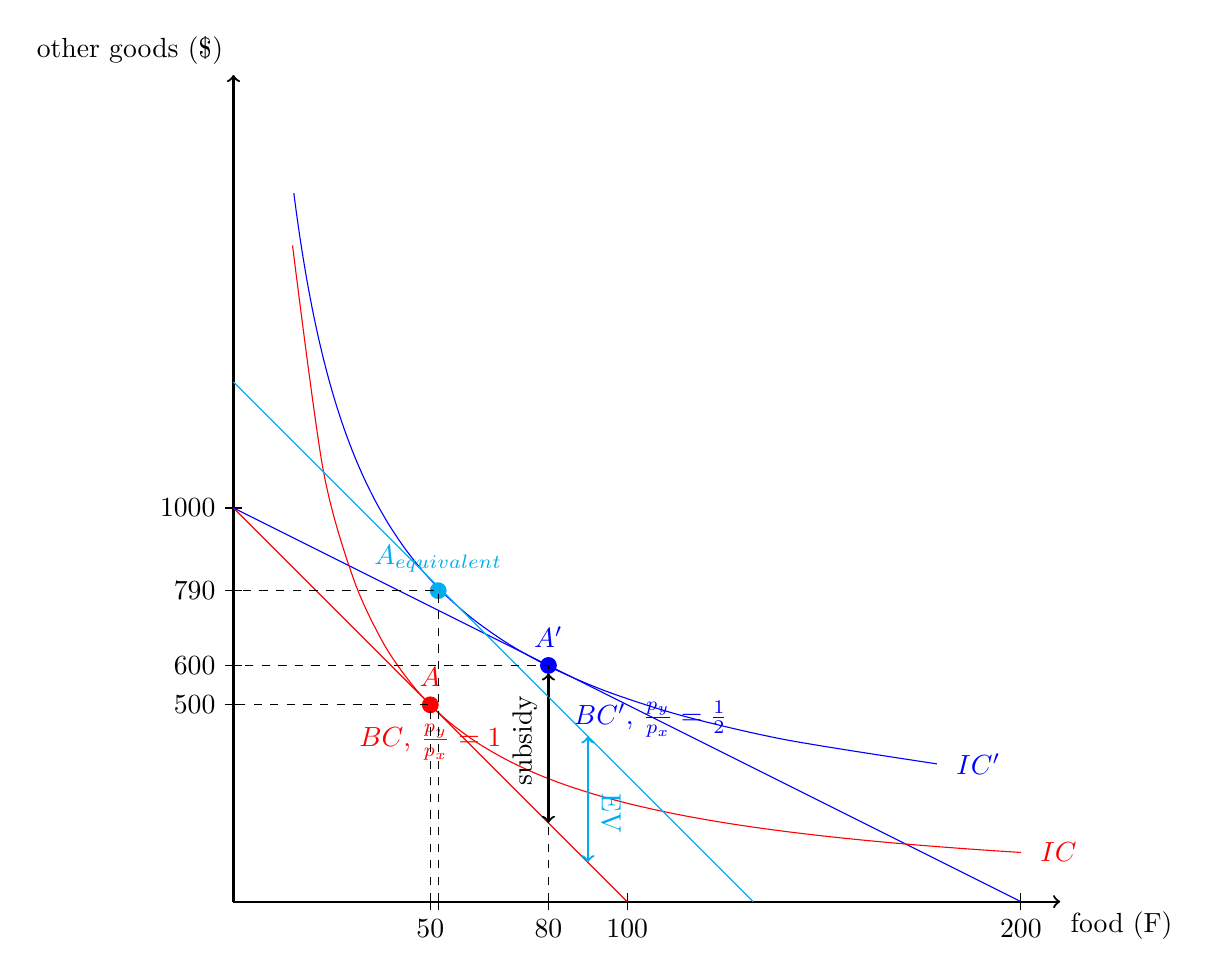
\begin{tikzpicture}[
    dot/.style={shape=circle, inner sep=2pt, draw, node contents=},
    circ/.style={shape=circle, inner sep=2pt, draw, fill}]
    \draw[thick,->] (0,0) -- (10.5,0) node[anchor=north west] {food (F)};
    \draw[thick,->] (0,0) -- (0,10.5) node[anchor=south east] {other goods (\$)};
    
    \draw (5cm,3pt) -- (5cm,-3pt) node[anchor=north] {$100$}; 
    \draw (2.5cm,3pt) -- (2.5cm,-3pt) node[anchor=north] {$50$}; 
    \draw (4cm,3pt) -- (4cm,-3pt) node[anchor=north] {$80$}; 
    \draw (10cm,3pt) -- (10cm,-3pt) node[anchor=north] {$200$}; 
    \draw (2.6cm,3pt) -- (2.6cm,-3pt) node[anchor=north] {}; 

    \draw (3pt,5cm) -- (-3pt,5cm) node[anchor=east] {$1000$};
    \draw (3pt,2.5cm) -- (-3pt,2.5cm) node[anchor=east] {$500$};
    \draw (3pt,3cm) -- (-3pt,3cm) node[anchor=east] {$600$};
    \draw (3pt,3.95cm) -- (-3pt,3.95cm) node[anchor=east] {$790$};

    \draw[color=red] (0,5) -- node[label=below:{$BC$, $\frac{p_y}{p_x} = 1$}]{} (5,0);
    \draw[color=blue] (0,5) -- node[label=below:{$BC'$, $\frac{p_y}{p_x} = \frac{1}{2}$},yshift=3mm,xshift=3mm]{} (10,0);


    \draw[color=red,domain=1.5:20,scale=0.5,smooth,variable=\x] plot ({\x},{25/\x}) node[label=right:{$IC$}]{};
    \draw[color=blue,domain=18:3.5,scale=0.5,smooth,variable=\x] plot ({117/sqrt(\x*\x*\x)}, {\x}) node[label=right:{$IC'$}]{};

    \draw[<->,thick] (4,1) -- node[rotate=90,xshift=8mm,yshift=3mm,left]{subsidy} (4,2.9);

    \draw[color=cyan] (0,6.6) -- (6.6,0);
    \draw[color=cyan,<->,thick] (4.5,0.5) -- node[rotate=270,xshift=-2mm,yshift=3mm,right]{EV} (4.5,2.1);
    \draw[color=red] (2.5,2.5) node[circ,label=above:{$A$}]{};
    \draw[color=cyan] (2.6,3.95) node[circ,label=above:{$A_{equivalent}$}]{};
    \draw[color=blue] (4,3) node[circ,label=above:{$A'$}]{};

    \draw[dashed] (2.5,0) -- (2.5,2.5) -- (0,2.5);
    \draw[dashed] (2.6,0) -- (2.6,3.95) -- (0,3.95);
    \draw[dashed] (4,0) -- (4,3) -- (0,3);
    
  \end{tikzpicture}
\end{center}

We can note that we have $EV$ less than the subsidy.

\subsection*{f)}

The fact that $EV$ is less than the subsidy means that a straight cash transfer
equal to $EV$ would've pushed utility to the same level as the subsidy for less
spending.

A benefit, however, to specific subsidies like the one on food here is that it
directly increases consumption of food even more than a straight cash transfer.
Thus, if the main goal is to reduce hunger drastically, it might wind up being
advantageous to directly subsidize food.

Also, people won't vote for direct cash transfers, so...

\section*{Problem 4}

\subsection*{a)}

The consumer's time constraint is $T = H + N$, where $H$ is the amount of time
spent working and $N$ is the amount of time not working.

\subsection*{b)}

The consumer's budget constraint is $pC = wH$, as they have no nonwage sources
of income.

\subsection*{c)}

Putting these together, we arrive at $pC = wT - wN$, or $pC + wN = wT$.

\subsection*{d)}

\subsubsection*{d.1}

\begin{align*}
  \Lag(C,N,\lambda) &= CN^2 - \lambda(pC + wN - wT) \\
\end{align*}

\subsubsection*{d.2}

\begin{align*}
  \frac{\delta \Lag}{\delta C} &= N^{*2} - p\lambda = 0\\
  \frac{\delta \Lag}{\delta N} &= 2C^*N^* - w\lambda = 0\\
  \frac{\delta \Lag}{\delta \lambda} &= pC^* + wN^* - wT = 0
\end{align*}

\subsubsection*{d.3}

\begin{alignat*}{2}
  && p\lambda &= N^{*2} \\
  && w\lambda &= 2C^*N^* \\
  &\implies& N^{*2} &= 2C^*N^*\frac{p}{w} \\
  &\implies& N^* &= \frac{2p}{w} C^* \\
  &\implies& 3pC^* &= wT \\
  &\implies& C^* &= \frac{wT}{3p} \\
  &\implies& N^* &= \frac{2T}{3} \\
  &\implies& \lambda &= \frac{4T^2}{9p}
\end{alignat*}

\subsection*{e)}

The labor supply is simply $H = T - N^* = \frac{T}{3}$.

\subsection*{f)}

Since $\frac{dH}{dw} = 0$, a wage increase has no effect on the amount worked.

\subsection*{g)}

Similarly, $\frac{dH}{dp} =0$, so they still would not work longer hours.

\subsection*{h)}

The time constraint remains the same, but the budget constraint becomes $pC = wH
- A = wT - wN - A \implies pC + wN = wT - A$.


\begin{alignat*}{2}
  && \Lag(C,N,\lambda) &= CN^2 - \lambda(pC + wN - wT + A) \\
  && \frac{\delta \Lag}{\delta C} &= N^{*2} - p\lambda = 0\\ 
  && \frac{\delta \Lag}{\delta N} &= 2C^*N^* - w\lambda = 0\\ 
  && \frac{\delta \Lag}{\delta \lambda} &= pC^* + wN^* - wT + A\\ 
  &\implies& p\lambda &= N^{*2} \\
  &\implies& w\lambda &= 2C^*N^* \\
  &\implies& N^{*2} &= 2C^*N^*\frac{p}{w} \\
  &\implies& N^* &= \frac{2p}{w} C^* \\
  &\implies& 3pC^* &= wT - A\\
  &\implies& C^* &= \frac{wT - A}{3p} \\
  &\implies& N^* &= \frac{2T}{3} - \frac{2A}{3w} \\
\end{alignat*}


\subsection*{i)}

In this case, we have that $H = T - N^* = \frac{T}{3} + \frac{2A}{3w}$. Thus,
$\frac{dH}{dw} = -\frac{2A}{3w^2} < 0$, so an increase in wages would lead to a
decrease in the time worked, approaching just $\frac{T}{3}$ hours worked as
wages grow large.

\subsection*{j)}

We still however have that $\frac{dH}{dp} = 0$, so inflation does not cause them
to work more or less.


\end{document}